\documentclass[11pt,fleqn]{article}

\setlength {\topmargin} {-.15in}
\setlength {\textheight} {8.6in}

\usepackage{amsmath}
\usepackage{amssymb}
\usepackage{color}
\usepackage{tikz}
\usetikzlibrary{automata,positioning,arrows}
\usepackage{diagbox}
\usepackage{stackrel}
\begin{document}


\textbf{Exercise 1.4.20:} Bitonic search. An array is bitonic if it is comprised of an increasing sequence
of integers followed immediately by a decreasing sequence of integers. Write a program
that, given a bitonic array of N distinct int values, determines whether a given integer
is in the array. Your program should use ~3lg N compares in the worst case.\\

\textbf{Solution:}
\begin{itemize}
	\item example array; [1,2,3,4,5,4,3,2]
	\item first, find bitonic point(the maximal/minimal point where an array starts increasing or decreasing on either side of it). We can do this using Binary Search.
	\item Search LHS and RHS of bitonic point to find the key.
	\item This results in 3 binary searches which means time complexity is $O(3logN)$
\end{itemize}

\newpage
\textbf{Pseudocode below}
\begin{center}
	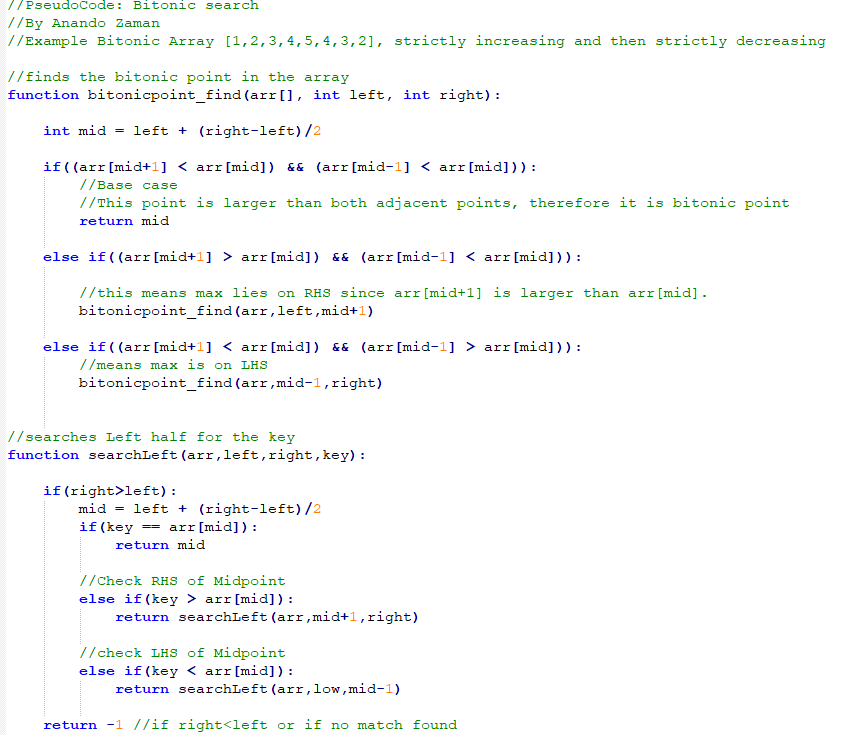
\includegraphics[scale = 1]{1.4.20.png}
	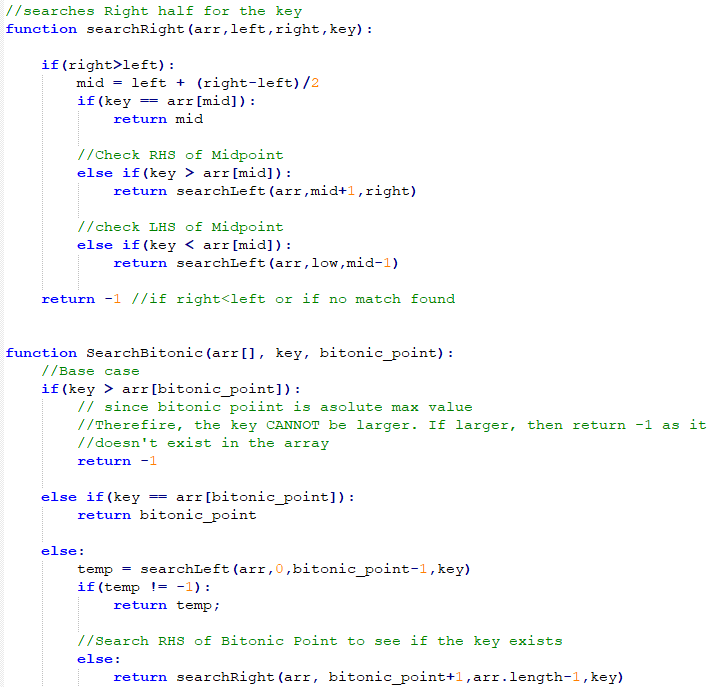
\includegraphics[scale = 1]{1.4.20-1.png}
	\end{center}

\end{document}
